% Source - https://tex.stackexchange.com/a/689563
% Posted by Qrrbrbirlbel
% Retrieved 2026-04-03, License - CC BY-SA 4.0

\documentclass[tikz]{standalone}
\usetikzlibrary{arrows.meta, graphs.standard, nfold}
\usetikzlibrary{spath3}
\makeatletter
\tikzset{
  offset round/.code=
    \tikz@addmode{%
      \pgfsetroundjoin         \pgfgetpath   \tikz@temp
      \pgfsetpath\pgfutil@empty\pgfoffsetpath\tikz@temp{#1}}}
\makeatother
\tikzset{
  vertex/.style={circle, inner sep=+0pt, minimum size=+2mm, draw},
  graphs/every graph/.append style={nodes=vertex, clockwise, typeset=}}
\begin{document}
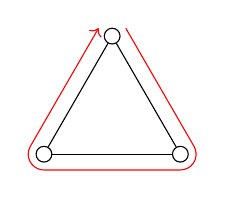
\begin{tikzpicture}
\graph[n=3]{subgraph C_n};
\draw[red, ->] plot[samples at={1, 2, 3, 1}] (\x) [offset round=2mm];
\end{tikzpicture}

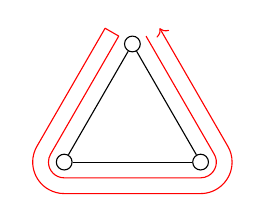
\begin{tikzpicture}
\graph[n=3]{subgraph C_n};
\path plot[samples at={1, 2, 3, 1}] (\x) [offset round=+ 2mm, spath/save=p];
\path plot[samples at={1, 3, 2, 1}] (\x) [offset round=+-4mm, spath/save=q];
\draw[->, red, spath/use=p] -- (spath cs:q 0) [spath/use={q, weld}];
\end{tikzpicture}

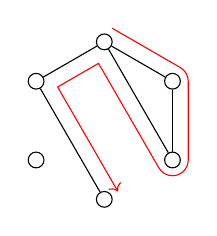
\begin{tikzpicture}
\graph[n=6]{subgraph I_n, 1 -- 2 -- 3 -- 1 -- 6 -- 4};
\draw[red, ->] plot[samples at={1, 2, 3, 1, 6, 4}] (\x) [offset round=2mm];
\end{tikzpicture}
\end{document}
